We seek the posterior distribution 
$\Prob(N, \ell, f | X)$. In most nontrivial probabilistic models, including ours, the exact posterior distribution is intractable.

Markov chain Monte Carlo (MCMC) is a common approach for approximating
posterior distributions by constructing a stochastic process on the parameter space whose stationary distribution is the exact posterior.
\jeff{Better to drop the word ``true'' here. There's the posterior distribution, and there are approximations to the posterior distribution.}
\bryan{I changed it to ``exact'' posterior; is that better?}
\jeff{It's better, but dropping ``exact'' may be better still. Feel free to ask Jon.}
However, its computational cost is prohibitively expensive for
large-scale astronomical surveys. Instead, we propose to construct an approximate posterior using variational inference, resulting in a procedure that is several orders of magnitude faster than MCMC.
\jeff{Probably better to move the comparison to MCMC to the introduction. Here we should just describe what we did with VI.}

Variational inference~\cite{Blei_2017_vi_review, Jordan_intro_vi, Wainwrite_graph_models_vi}
posits a family of distributions $\mathcal{Q}$ and seeks
the distribution $q^*\in \mathcal{Q}$ that is closest to the exact posterior
in $\KL$ divergence. Suppose the family of distributions $\mathcal{Q}$ is parameterized by a real-valued vector $\eta$. The objective is 
\begin{align}
   \eta^* &= \argmin_{\eta} \Big\{ \mathrm{KL}\Big[\,q_\eta(N, \ell, f | X)\, \| \,p(N, \ell, f | X )\,\Big]\Big\} 
   \label{eq:kl_objective}
\end{align}

Minimizing the $\KL$ divergence is equivalent to maximizing the ELBO (evidence lower bound), defined as 
\begin{align}
    \mathcal{L} = 
    \Expect_{q_\eta(N, \ell, f | X)}\Big[\log p(X, N, \ell, f) - \log q_\eta(N, \ell, f | X)\Big].
    \label{eq:elbo}
\end{align}
The ELBO does not depend on the intractable marginal distribution $p(X)$.

\subsection{The variational distribution}
% We now describe our family of distributions $\mathcal{Q}$. 
In the traditional variational inference setup, 
$q_\eta$ depends on data $X$ only through the optimization objective 
(so $q_\eta(N, \ell, f | X)$,
becomes $q_\eta(N, \ell, f)$ with no dependence on $X$). 
Here, we take an amortized approach where
$q_\eta$ explicitly depends on data $X$. Specifically, a neural network 
maps input data $X$ to distributional parameters of $(N, \ell, f)$ 
under $q$. The variational parameters $\eta$ in equation~\eqref{eq:kl_objective} 
are the neural network weights. 
In the ensuing subsections, we detail the construction of our variational distribution. 

\subsubsection{The factorization}
To make the objective in \eqref{eq:kl_objective} tractable in most 
applications, the family $\mathcal{Q}$ is restricted to probability distributions 
that limit conditional dependencies between latent variables. In the most extreme case, mean-field variational inference, 
the distribution over latent variables is assumed to fully factorize in the approximate posterior. 

Our factorization takes a spatial structure: we decompose the full $H \times W$ image into disjoint $S \times S$ tiles. Explicitly, each tile $\tilde x_{rs}$ is comprised of pixels 
\begin{align}
    \tilde x_{rt} = \{x_{hw} : S(r+1) \geq h > Sr \text{ and } S(t+1) \geq w > St\}.
\end{align}
for $r = 1, ..., \frac{H}{S}$ and $t = 1, ..., \frac{W}{S}$ (we assume that $H$ and $W$ are multiples of $S$). See Figure~\ref{fig:ex_tiles} for a schematic. 
% \jeff{Also, we should define what tiles are.}
% \jeff{The dimension of the tiles maybe better in uppercase: the other ``structural constants'' are uppercase (e.g., $H$, $W$).}
There is a function that maps 

Let $N_{rt}$ be the number of stars in tile $r, t$. 
On each tile, we also construct a triangular array of 
locations and fluxes:
\begin{align}
    \tilde\ell^{(r,t)} &= (\tilde\ell_{N, i}^{(r,t)} : i = 1, ..., N; N = 1, 2, ...) \\
    \tilde f^{(r,t)} &= (\tilde f_{N, i}^{b, (r,t)} : 
    b = 1, ..., B; i = 1, ..., N; N = 1, 2, ...)
\end{align}
There is a mapping from latent variables on each tile to latent variables on the full image 



Let $k = 1, ..., K$ index the tiles. Then
denote the number of stars on tile $k$ by $N^{(k)}$;
the locations by $\ell^{(k)} = (\ell_{N, i}^k)_{i \leq N}$; 
the fluxes $f^{(k)} = (f_{N, i}^k)_{i \leq N}$. Our variational 
distribution factorizes over image tiles, so
\begin{align}
    q\big((N^{(k)}, \ell^{(k)}, f^{(k)})_{k = 1}^K|X\big) = \prod_{k = 1}^K q_\eta\big(N^{(k)}, \ell^{(k)}, f^{(k)} | X\big). 
\end{align}
\jeff{Probably $q$ should have $\eta$ as a subscript on the lhs too}

\begin{figure}[h]
    \centering
    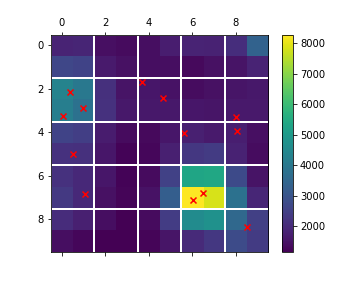
\includegraphics[width = 0.5\textwidth]{figures/example_tiled.png}
    \vspace{-1cm}
    \caption{Tiling a 10 x 10 image into 2 x 2 tiles.}
    \label{fig:ex_tiles}
\end{figure}
\jeff{Would you want to introduce a term like ``padded tiles'' somewhere to refer to the tile plus some of the nearby pixels around it? Tiles are disjoint from each other but padded tiles overlap some with each other.}

There is a bijection between latent variables on each tile and latent variables on the full image (locations on the full image map to locations on image tiles and vice-versa). 
\jeff{It's not clear what it means for a latent variable to be ``on a tile''. Why a bijection? They're the same latent variables, right?}
Thus, a variational distribution for latent variables on tiles induces a variational distribution for latent variables on the full image.
\jeff{This isn't such a good way to explain it. Better to directly explain the variational distribution over the whole image, from top down, introducing the concept of tiles along the way. Perhaps at the end make the point that our choice of variational distribution does not render the problem embarrassingly parallel.}
Let $T$ be the mapping from latent variables on tiles to latent variables on the full image. Then, the variational distribution for the latent variables is
\begin{align}
    (N, \ell, f) &\stackrel{d}{=} T((N^{(k)}, \ell^{(k)}, f^{(k)})_{k = 1}^K), \notag \\  
        &\text{where } (N^{(k)}, \ell^{(k)}, f^{(k)})_{k = 1}^K \sim \prod_{k = 1}^K q_\eta(N^{(k)}, \ell^{(k)}, f^{(k)} | X). 
\end{align}
\jeff{I suggest getting rid of $T$ here. This bijection is a confusing way to explain things. Instead, to refer to the pixels in tile (i, j), you might define
\[
    \tilde x_{i,j} = \{x_{hw} : Si \ge h > S(i + 1) \text{ and } Sj \ge w > S(j+1)\}.
\]
You could do the same thing for $\tilde f$, etc.
}
\jeff{Is there somewhere you say that in the variational distribution, $N = \sum_{k=1}^K N^{(k)}$ ? That might be a good way to put it.}

\subsubsection{Distributions on image tiles}
We describe the distribution on each tile, $q_\eta(N^{(k)}, \ell^{(k)}, f^{(k)} | X)$. 
Dropping the tile index $k$ in this subsection,
\jeff{It seems confusing to me to drop the index $k$ here: earlier $N$ without a $(k)$ superscript meant something else.}
\begin{align}
    N &\sim \text{Categorical}(\omega; 0, ..., N_{max}) \label{eq:var_distr_n}\\
	\ell_{N, i} / s &\sim \text{LogitNormal}(\mu_{\ell_{N, i}}, \text{diag}(\nu_{\ell_{N, i}}) )\label{eq:var_distr_loc}\\
	f^b_{N, i} &\sim \text{LogNormal}(\mu_{f^b_{N, i}}, \sigma^2_{f^b_{N, i}}) \label{eq:var_distr_f}
\end{align}
for $i = 1, ..., N$; $N = 1, ..., N_{max}$. The latent variables also fully factorize within each tile. Note that in the exact posterior, $N$ has support on the nonnegative integers; in practice, we truncate at an $N_{max}$ large.
\jeff{Do we? I thought it was just the variational distribution that doesn't have support past $N_{max}$. The posterior has support over all natural numbers.}


These distributions were taken for convenience: fluxes are positive and right skewed, so we place a normal distribution on log-fluxes; locations are between zero and $s$, so 
we place a normal distribution on the logit of the location scaled by $1 / s$. 

\subsubsection{Neural network architecture}
On each tile, the parameters of the variational distribution, \eqref{eq:var_distr_n}-\eqref{eq:var_distr_f}, are the output of a neural network.
\jeff{The parameters of the variational distribution are the weights of the neural network, not the outputs.}
The input to the neural network is the $s \times s$ tile, padded with surrounding pixels.
For cataloging the crowded starfield M2,
we took $s = 2$ and padded the tile with three pixels. 
For our test on a sparse field, we took $s = 50$ with no padding. 
The architecture is shown schematically in Figure~\ref{fig:starnet_arch}. 

\begin{figure}[!h]
    \centering
    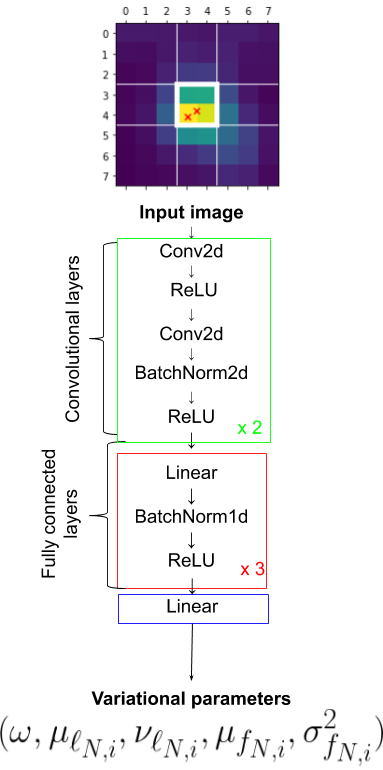
\includegraphics[width=0.4\textwidth]{figures/starnet_archetecture2.png}
    \vspace{-0.5cm}
    \caption{For cataloging M2, the neural network returning parameters for the variational distribution on each 2 x 2 image tile.
    On a sparse field, the neural network architecture is the same, 
    except the input is a $50 \times 50$ image tile. }
    \label{fig:starnet_arch}
\end{figure}

Consider the output dimension of the neural network. The categorical parameter $\omega$ lies on the 
simplex and has dimension $N_{max} + 1$; for each $i = 1, ..., N$ and $N = 1, ..., N_{max}$, the location has a mean and variance on each coordinate; the flux has a mean and variance for each band. Thus, for star indexed by $(i, N)$, 
there are $2 \times (B + 2)$ parameters for its variational distribution. In total, the neural network has output dimension $(N_{max} + 1) + (B + 2) \times (N_{max}^2 + N_{max})$. 

Recall that locations on the 
full image $\ell_{N, i}$ are parameterized to be in $[0, H] \times [0, W]$. 
On the tiles, locations $\ell^{(k)}_{N, i}$ are parameterized to be in
$[0, s] \times [0, s]$. 

Thus, decomposing the inference problem from full images into $2 \times 2$ tiles
\jeff{What does it mean to decompose an inference problem from full images into tiles?}
controls the output dimension of the neural network. 
On a crowded starfield with $H = W = 100$, $N$ is on the order of $10^3$, 
\jeff{I'd say ``the number imaged of stars'' here rather than $N$, because $N$ (unlike $H$ and $W$) is random variable in our model, and we're describing the data.}
and $N_{max}$ must be larger. 
On the $2\times 2$ tile, we set $N_{max} = 3$. 
Moreover, the tiling amortizes the inference across image tiles: the same neural network is reused for each tile. 

While the variational distribution factorizes over $2 \times 2$ tiles, we are not breaking the inference problem on the full image into embarrassingly parallel subproblems. We always evaluate the likelihood (when example, when computing the ELBO, equation~\eqref{eq:elbo}) on the full image.
Light from a star within a 2 x 2 tile spills over into neighboring tiles, so the likelihood does not decouple into image tiles. 
